\documentclass[letterpaper,spanish,10pt]{article}
\usepackage[latin1]{inputenc}    % Agregar y acentos
\usepackage{babel}               % Soporte multilenguajes
\usepackage{avant}               % Tipo de fuente
%\usepackage{fancyheadings}       %% Topes y pies de pï¿œina
\usepackage[dvips]{graphicx}     % Inclusion de imagenes .eps
\usepackage{url}                 % Agregar Links soporte de ~
\usepackage{verbatim}
\usepackage{geometry}
\usepackage{url}
\usepackage{amsfonts}
\usepackage{amssymb}
%\usepackage{txfonts}
%\usepackage{emphoff}
%\usepackage{pxfonts}
%\usepackage{fancybox}
\usepackage{latexsym}
%\usepackage{fancyvrb}
\usepackage{graphicx}
%\usepackage{wasysym}
%\renewcommand{\baselinestretch}{1.5}
\parskip=7mm
\pagestyle{myheadings}
\geometry{tmargin=2.5cm, bmargin=2.5cm, lmargin=2.5cm, rmargin=2.5cm}
\markright{\hrulefill Proyecto Hevelius $\; \;$}


%opening
\title{{\Huge \bf Proyecto Hevelius} \\ {\Large Empresa DevNull} \\ {\small Riesgos (Parte 2)}}

\author{
{\bf Carlos Guajardo Miranda} \\ Jefe de Proyecto \\ \url{cguajard@alumnos.inf.utfsm.cl} \\ cel. 09-95046118 
\and
{\bf Marina Pilar Daza} \\ Miembro del Equipo \\ \url{mpilar@alumnos.inf.utfsm.cl} \\ cel. 09-84085407
\and
{\bf Esteban Espinoza Mart\'inez} \\ Miembro del Equipo \\ \url{eespinoz@alumnos.inf.utfsm.cl} \\ cel. 09-85596939
\and
{\bf Tom\'as Staig Fern\'andez} \\ Miembro del Equipo \\ \url{tstaig@alumnos.inf.utfsm.cl} \\ cel. 09-97615666
}


\date{27 de abril de 2007}


\begin{document}

\maketitle
%\tableofcontents


%\input{parte1}
%\input{parte2}
\newpage



\section{Modelo de Casos de Uso}

\begin{figure}[h]
  \centering
    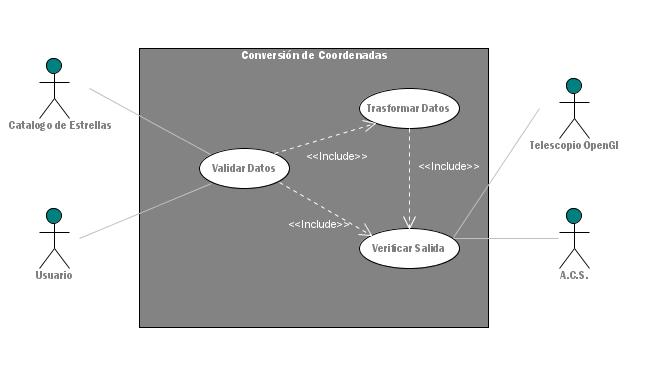
\includegraphics[width=7in]{modelo}
\end{figure}



\section{Contratos derivados de los casos de uso de la transformaci\'on de las coordenadas}

\subsection{Descripci\'on Caso de Uso}

\begin{itemize}
\item \textbf{Nombre:} Validar Datos.
\item \textbf{Actores:} Catalogo de Estrellas y usuarios.
\item \textbf{Descripci\'on:} Consiste en la verificaci\'on de datos, para que sean caracteres validos para le sistema.
\item \textbf{Funci\'on:} Verificar coherencia de datos.
\end{itemize}

\subsection{Subcasos de Uso}

\begin{itemize}
\item \textbf{Nombre:} Transformaci\'on.
\item \textbf{Actores:} Catalogo de Estrellas y usuarios.
\item \textbf{Funcion:} Conversi\'on de datos a coordenadas horizontales.
\item \textbf{Descripci\'on:} Cuando se ingresan coordenadas R.A.Dec, ya sea de usuario o catalogo, se convierte en coordenadas horizontales.
\end{itemize}

\begin{itemize}
\item \textbf{Nombre:} Verificaci\'on de Salida.
\item \textbf{Actores:} Catalogo de Estrellas y usuarios.
\item \textbf{Funci\'on:} Verifica que no se entregen coordenadas invalidas.
\item \textbf{Descripci\'on:} Luego de comprobar que solo se ingresaron valores coherentes, se verifica que estas coordenadas sean validas, por ejemplo que estas no apunten a objetos celestes que esten al otro lado de la ubicaci\'on actual.
\end{itemize}


\subsection{Contratos}

\begin{itemize}
\item \textbf{Nombre:} \url{public boolean validar\_datos(double coord1, double coord2)}
\item \textbf{Responsabilidad:} Verific\'ar que los valores ingresados sean coherentes. Discriminar si los datos de entrada corresponden a R.A.Dec u Horizontal.
\item \textbf{Salida:} Valor boolean que retorna exito o fracaso seg\'un sean datos coherentes.
\item \textbf{Postcondici\'on:} En caso de \'exito entrga un dato dependiendo del tipo de coordenadas a ``Transformaci\'on'' o a ``Verificar Sal\'ida''.
\item \textbf{Precondicion:} Que los datos ingresados sean n\'umeros double, no nulos.
\end{itemize}

\begin{itemize}
\item \textbf{Nombre:} \url{public void transformar(double cood1, double coord2)}
\item \textbf{Responsabilidad:} Convertir las coordenadas R.A.Dec a Horizontales.
\item \textbf{Salida:} No retorna nada.
\item \textbf{Postcondici\'on:} Entrega los datos a ``verificaci\'on''.
\item \textbf{Precondici\'on:} Coordenadas en formato R.A.Dec.
\end{itemize}

\begin{itemize}
\item \textbf{Nombre:} \url{public boolean verificar(double coord1, double coord2)}
\item \textbf{Responsabilidad:} Verificar que las coordenadas no apunten a una ubicaci\'on inalcanzable como en una direci\'on al otro lado de la tierra.
\item \textbf{Salida:} Valor boolean que indica si es accsesible o no la ubicaci\'on.
\item \textbf{Postcondici\'on:} Entrga los datos al sistema de telescopio OpenGL y ACS para la manipulaci\'on del telescopio (en caso de exito, si no avisa para volver a intentar).
\item \textbf{Precondici\'on:} Coordenadas en formato Horizontal.
\end{itemize}


\section{Investigaci\'on de las Coordenadas}













\end{document}
